\documentclass[12pt,]{article}
\usepackage{lmodern}
\usepackage{amssymb,amsmath}
\usepackage{ifxetex,ifluatex}
\usepackage{fixltx2e} % provides \textsubscript
\ifnum 0\ifxetex 1\fi\ifluatex 1\fi=0 % if pdftex
  \usepackage[T1]{fontenc}
  \usepackage[utf8]{inputenc}
\else % if luatex or xelatex
  \ifxetex
    \usepackage{mathspec}
  \else
    \usepackage{fontspec}
  \fi
  \defaultfontfeatures{Ligatures=TeX,Scale=MatchLowercase}
\fi
% use upquote if available, for straight quotes in verbatim environments
\IfFileExists{upquote.sty}{\usepackage{upquote}}{}
% use microtype if available
\IfFileExists{microtype.sty}{%
\usepackage{microtype}
\UseMicrotypeSet[protrusion]{basicmath} % disable protrusion for tt fonts
}{}
\usepackage[margin=1in]{geometry}
\usepackage{hyperref}
\hypersetup{unicode=true,
            pdftitle={Efectividad de reservas marinas a nivel nacional},
            pdfauthor={Juan Carlos Villaseñor-Derbez, Stuart Fulton, Jorge Torre},
            pdfborder={0 0 0},
            breaklinks=true}
\urlstyle{same}  % don't use monospace font for urls
\usepackage{graphicx,grffile}
\makeatletter
\def\maxwidth{\ifdim\Gin@nat@width>\linewidth\linewidth\else\Gin@nat@width\fi}
\def\maxheight{\ifdim\Gin@nat@height>\textheight\textheight\else\Gin@nat@height\fi}
\makeatother
% Scale images if necessary, so that they will not overflow the page
% margins by default, and it is still possible to overwrite the defaults
% using explicit options in \includegraphics[width, height, ...]{}
\setkeys{Gin}{width=\maxwidth,height=\maxheight,keepaspectratio}
\IfFileExists{parskip.sty}{%
\usepackage{parskip}
}{% else
\setlength{\parindent}{0pt}
\setlength{\parskip}{6pt plus 2pt minus 1pt}
}
\setlength{\emergencystretch}{3em}  % prevent overfull lines
\providecommand{\tightlist}{%
  \setlength{\itemsep}{0pt}\setlength{\parskip}{0pt}}
\setcounter{secnumdepth}{0}
% Redefines (sub)paragraphs to behave more like sections
\ifx\paragraph\undefined\else
\let\oldparagraph\paragraph
\renewcommand{\paragraph}[1]{\oldparagraph{#1}\mbox{}}
\fi
\ifx\subparagraph\undefined\else
\let\oldsubparagraph\subparagraph
\renewcommand{\subparagraph}[1]{\oldsubparagraph{#1}\mbox{}}
\fi

%%% Use protect on footnotes to avoid problems with footnotes in titles
\let\rmarkdownfootnote\footnote%
\def\footnote{\protect\rmarkdownfootnote}

%%% Change title format to be more compact
\usepackage{titling}

% Create subtitle command for use in maketitle
\newcommand{\subtitle}[1]{
  \posttitle{
    \begin{center}\large#1\end{center}
    }
}

\setlength{\droptitle}{-2em}
  \title{Efectividad de reservas marinas a nivel nacional}
  \pretitle{\vspace{\droptitle}\centering\huge}
  \posttitle{\par}
\subtitle{Casos de estudio del Pacífico, Golfo de California, y Sistema Arrecifal
Mesoamericano}
  \author{Juan Carlos Villaseñor-Derbez, Stuart Fulton, Jorge Torre}
  \preauthor{\centering\large\emph}
  \postauthor{\par}
  \date{}
  \predate{}\postdate{}

\usepackage{booktabs}
\usepackage{longtable}
\usepackage{array}
\usepackage{multirow}
\usepackage[table]{xcolor}
\usepackage{wrapfig}
\usepackage{setspace}
\doublespacing

\begin{document}
\maketitle

{
\setcounter{tocdepth}{2}
\tableofcontents
}
\section{Resumen ejecutivo}\label{resumen-ejecutivo}

\section{Introducción}\label{introduccion}

La sobrepesca y prácticas pesqueras no sostenibles son unas de las
mayores amenazas para la conservación de los ecosistemas marinos del
mundo (Halpern et al., 2008, 2017). La implementación de reservas
marinas (\emph{i.e.} áreas donde la captura de una o más especies está
prohibida) es una medida de manejo frecuentemente propuesta para
recuperar stocks pesqueros e impulsar la productividad pesquera en aguas
cercanas (Afflerbach et al., 2014; Krueck et al., 2017; Sala \&
Giakoumi, 2017). Recientes trabajos han demostrado que también pueden
mitigar y proveer amortiguamiento ante el cambio climático (Roberts et
al., 2017), variabilidad ambiental (Micheli et al., 2012), resolver
problemas de pesca incidental (Hastings, Gaines \& Costello, 2017) y, en
general, incrementar la biomasa, riqueza y densidades de organismos
dentro de sus fronteras (Lester et al., 2009; Giakoumi et al., 2017;
Sala \& Giakoumi, 2017).

En México, las reservas marinas han sido comúnmente establecidas como
zonas núcleo dentro de Reservas de la Biósfera (RBs), administradas por
la Comisión Nacional de Áreas Naturales Protegidas (CONANP). Al día de
hoy, \textbf{41} RBs protegen una porción del ambiente marino en México.
Sin embargo, solamente \textbf{27} de estas incluyen (pequeñas) zonas
núcleo donde las actividades pesqueras están prohibidas. Aunque la
CONANP ha hecho esfuerzos importantes por involucrar a los actores
durante la implementación de las reservas, esto aún se caracteriza por
un proceso descendente, el cual conlleva a la falta de cumplimiento por
parte de los actores. La escasez de recursos monetarios y humanos de la
limitan también el monitoreo y vigilancia de las reservas, y a su vez,
el desempeño de la reserva.

Buscando promover una alternativa con procesos ascendentes para
implementar reservas marinas, las OSCs comenzaron a trabajar con
comunidades pesqueras para establecer reservas comunitarias (Uribe et
al., 2010) . Estas son comúnmente establecidas dentro de zonas de
concesión, una forma de derechos de uso territoriales para pesquerías
(TURF, en inglés). Al permitir a los pescadores diseñar sus propias
reservas, una mayor proporción de la comunidad está de acuerdo con los
perímetros y reglas establecidas, y por lo tanto los respetan (Beger et
al., 2004; Espinosa-Romero et al., 2014; Gelcich \& Donlan, 2015) .
Adicionalmente, los pescadores pueden implementar sus reservas por un
periodo acordado (usualmente cinco años), después del cual la reserva
puede ser abierta a la pesca. Esto provee a los pescadores con un
sentido de confianza de que, en caso de ser necesario, aún tienen acceso
a pescar esa zona\footnote{Hasta ahora, solamente una comunidad ha
  decidido abrir sur reservas a la pesca.}. Las reservas son
directamente vigiladas y monitoreadas por la comunidad, quienes
comúnmente utilizan pequeñas embarcaciones (\emph{e.g.} pangas) para
patrullar la zona, o realizan avistamientos desde la costa en búsqueda
de pescadores ilegales Aún así, las reservas comunitarias carecen de
reconocimiento legal; por lo tanto, no hay forma de penalizar a los
infractores.

Sin embargo, en el 2014 una nueva norma (NOM-049-SAG/PESC, 2014) permite
a los pescadores solicitar el establecimiento de reservas marinas bajo
el nombre de ``Zonas de refugio Pesquero'' (ZRP). El manejo de las ZRP
combina procesos ascendentes y descendentes al reconocer legalmente las
reservas propuestas por las comunidades. Posterior a la revisión por
parte de la Comisión Nacional de Acuacultura y Pesca (CONAPESCA) y la
opinión técnica del Instituto Nacional de Acuacultura y Pesca (INAPESCA)
las ZRP son establecidas por el periodo solicitado por los
pescadores\footnote{Existen excepciones a esto, como la ``Zona de
  Refugio Pesquero Golfo de Ulloa'' y la ``Zona de Refugio Pesquero
  Akumal'', creadas por CONAPESCA para cerrar la pesca y prevenir la
  captura incidental de tortugas marinas.} . El monitoreo y la
vigilancia de las ZRP es típicamente llevado a cabo por la comunidad ,
con ayuda de OSCs locales. Hasta este cambio regulatorio, las reservas
comunitarias no contaban con el soporte legal, y eran solamente
reconocidas por la comunidad. Al día de hoy, existen \textbf{35} ZRP
establecidas en el Pacífico, Golfo de California y Caribe Mexicano.

Aunque existen tres aproximaciones generales para implementar reservas
marinas en México (\emph{i.e.} Zonas núcleo dentro de AMP, reservas
comunitarias y Zonas de Refugio Pesuqero), aún no comprendemos a fondo
las características sociales que permiten su efectividad. La ciencia de
reservas marinas se ha enfocado ampliamente en los efectos biológicos
que estas tienen (Lester et al., 2009; Afflerbach et al., 2014; Giakoumi
et al., 2017; Krueck et al., 2017; Sala \& Giakoumi, 2017). Aunque el
aspecto ecológico de las reservas es importante para su éxito, su
efectividad también depende del estado socioeconómico y los sistemas de
gobernanza de las comunidades pesqueras.

La literatura indica que diferentes características influyen en el éxito
de una reserva. En Palau, por ejemplo, la edad (\emph{i.e.} tiempo
transcurrido desde implementación), tamaño y hábitat contenido son
características claves que determinan la efectividad (Friedlander et
al., 2017). Por otro lado, en el Mar Meditarráneo, Di Franco et al.
(2016) identifican que la procuración y vigilancia, presencia de un plan
de manejo, participación de pescadores en el manejo, representación de
pescadores en la toma de decisiones y promoción de la pesca sustentable
son los cinco factores que incrementan la salud de los stocks y el
ingreso económicos a los pescadores, a la vez que se presenta una mayor
aceptación social de las prácticas de manejo. En una aproximación
global, Edgar et al. (2014) encuentran que la procuración, edad, tamaño
y aislamiento son determinantes de la efectividad de las reservas. Por
lo tanto, observamos que las características que habilitan el éxito
varían a través de regiones, y poco esfuerzo se ha hecho por comprender
estas interacciones en México.

\section{Objetivos}\label{objetivos}

El objetivo de este trabajo este trabajo es realizar una evaluación de
la efectividad de reservas marinas en México, presentando resultados de
cinco comunidades costeras como caso de estudio. Las comunidades
utilizadas en este reporte se distribuyen a lo largo de la costa
Pacífica de Baja Claifornia, el Golfo de California, y el Sistema
Arrecifal Mesoamericano. Con el fin de obtener una visión holística del
sistema, la evaluación se realizará tomando en cuenta indicadores
biológicos, socioeconómicos y de gobernanza (\textbf{Referencia aqui}).

La evaluación de éstos cinco casos de estudios nos permitirá identificar
l amanera en que las características socioeconómicas y de gobernanza se
relacionan con la efectividad (biológica) de las reservas marinas
evaluadas. Los patrones identificados podrán utilizarse para informar la
toma de desiciones para la implementación de la red de reservas marinas
en la Región de las Grandes Islas del Golfo de California.

\section{Métodos}\label{metodos}

\subsection{Zonas de estudio}\label{zonas-de-estudio}

\begin{itemize}
\tightlist
\item
  Maria Elena
\item
  Punta Herrero
\item
  Isla Natividad
\item
  Guaymas
\item
  Puerto Libertad (Cerro bola)
\end{itemize}

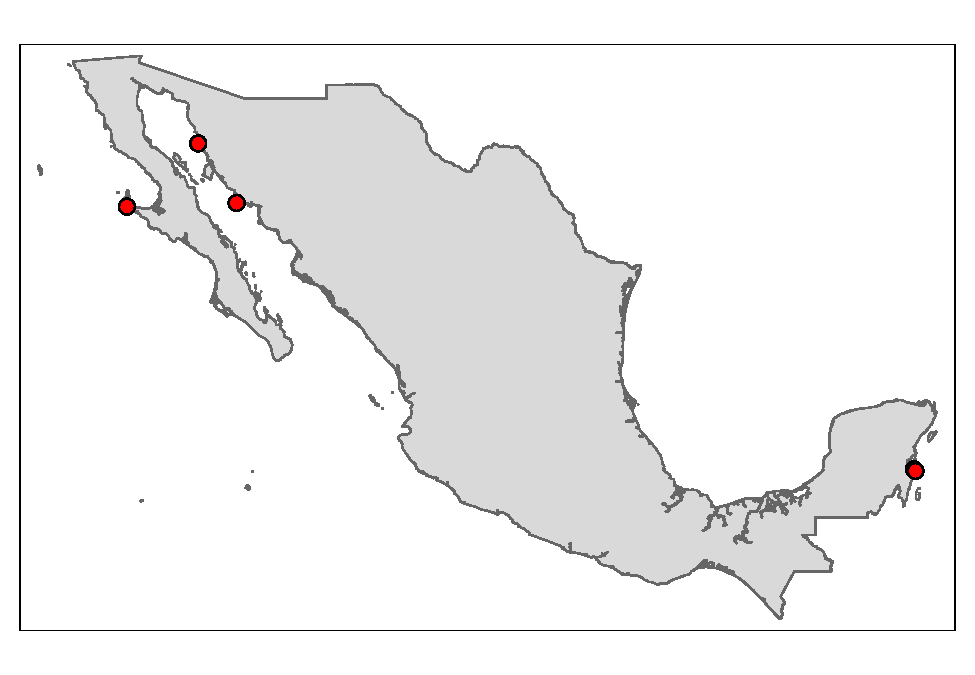
\includegraphics{Manuscript_files/figure-latex/unnamed-chunk-2-1.pdf}

\subsection{Datos y análisis de datos}\label{datos-y-analisis-de-datos}

Para evaluar las reservas, utilizamos tres fuentes de información. La
información ecológica proviene de los monitoreos ecológicos realizados
anualmente en las zonas reserva y control. Cada año, se realizan censos
visuales para evaluar las comunidades de peces e invertebrados,
registrando riquezas, abundancias y tallas (en peces). Esta información
nos permite calcular los indicadores biológicos. La información
socioeconómica proviene de los avisos de arribo de CONAPESCA. En este
caso, se tienen registros mensuales de cada una de las especies
aprovechadas por las diferentes comunidades, en los que se reportan los
arribos (Kg) y el valor de los arribos (\$). Los ingresos generados por
arribos son ajustados por medio del índice de precio al consumidor. La
información de governanza fue obtenida a nivel de comunidad, pidiendo a
personas familiares con las comunidades que proveyeran la información
necesaria.

Dada la similitud de objetivos entre las reservas, la evaluación se
realiza con los mismos indicadores. En este caso, se utilizan nueve
indicadores biológicos, 4 socioeconómicos y 14 de gobernanza.

\begin{table}

\caption{\label{tab:unnamed-chunk-3}Lista de indicadores utilizados para evaluar resvas marinas, agrupados por tipo.}
\centering
\begin{tabular}[t]{l}
\toprule
Indicador\\
\midrule
\addlinespace[0.5em]
\multicolumn{1}{l}{\textbf{Biológicos}}\\
\hspace{1em}Índice de diversidad de shannon\\
\hspace{1em}Riqueza\\
\hspace{1em}Densidad\\
\hspace{1em}Nivel trófico\\
\hspace{1em}Biomasa\\
\addlinespace
\addlinespace[0.5em]
\multicolumn{1}{l}{\textbf{Socioeconómicos}}\\
\hspace{1em}Ingresos\\
\hspace{1em}Arribos\\
\hspace{1em}Ingresos por especies objetivo\\
\addlinespace[0.5em]
\multicolumn{1}{l}{\textbf{Gobernanza}}\\
\hspace{1em}\hspace{1em}Arribos de especies objetivo\\
\hspace{1em}Acceso a la pesqueria\\
\addlinespace
\hspace{1em}Numero de pescadores\\
\hspace{1em}Reconocimiento legal de la reserva\\
\hspace{1em}Tipo de reserva\\
\hspace{1em}Grado de pesca ilegal\\
\hspace{1em}Plan de manejo\\
\addlinespace
\hspace{1em}Procuracion de la reserva\\
\hspace{1em}Tamano de la reserva\\
\hspace{1em}Razonamiento para el diseno de la reserva\\
\hspace{1em}Pertenencia a oragnizaciones pesqueras\\
\hspace{1em}Tipo de organizacion pesquera\\
\addlinespace
\hspace{1em}Representacion\\
\hspace{1em}Reglamentacion interna\\
\hspace{1em}Efectividad percibida\\
\bottomrule
\end{tabular}
\end{table}

Dado que el interés principal de este trabajo es identificar las
relaciones entre la efectividad de una reserva y las características
socioeconómicas y de gobernanza de su comunidad, los análisis se
realizan a nivel de comunidad, agrupando los datos para todas las
reservas y sitios control. Sin embargo, para controlar por respuestas
diferenciales de cada sitio (para comunidades con más de una reserva),
debemos tomar en cuenta factores específicos a cada sitio. Para esto,
modificamos el modelo de diferencia en diferencias utilizado para
indicadores biológicos agregándo el término para sitio de la siguiente
manera:

\[I = \beta_0 + \sum \gamma Ano + \beta_1 Zona + \beta_2 Post\times Zona + \beta_3Sitio + \epsilon\]

\section{Resultados}\label{resultados}

\subsection{Isla Natividad}\label{isla-natividad}

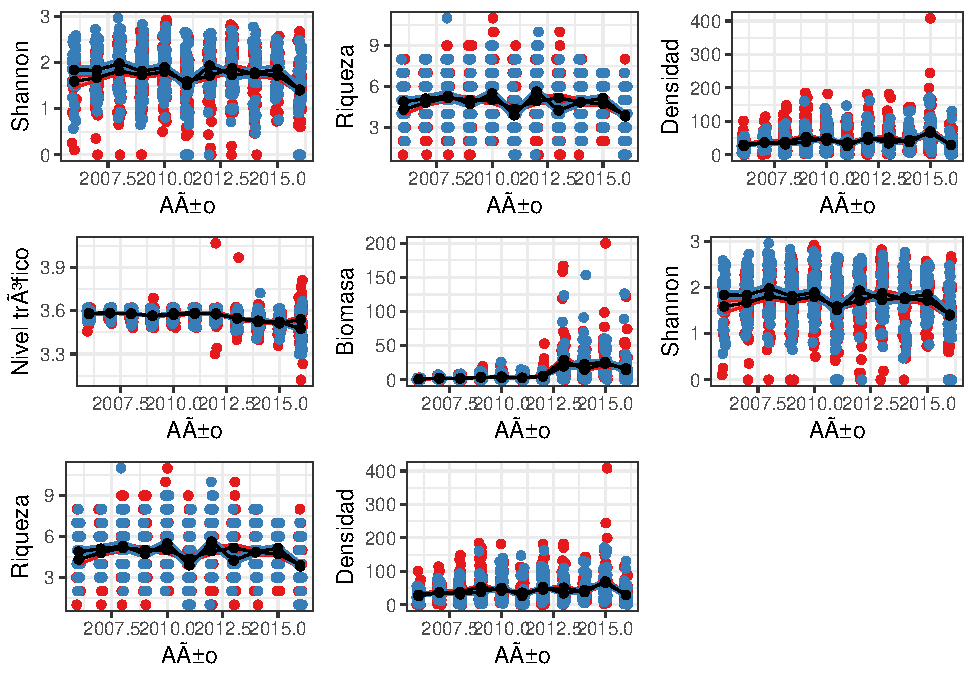
\includegraphics{Manuscript_files/figure-latex/unnamed-chunk-7-1.pdf}

\subsection{Puerto Libertad}\label{puerto-libertad}

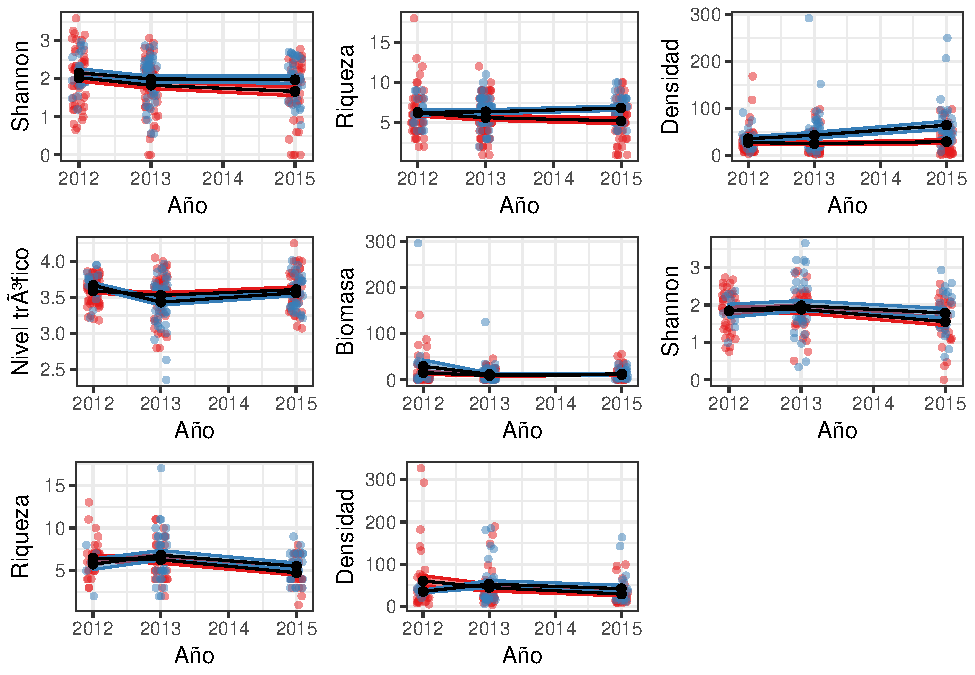
\includegraphics{Manuscript_files/figure-latex/unnamed-chunk-8-1.pdf}

\subsection{Guaymas}\label{guaymas}

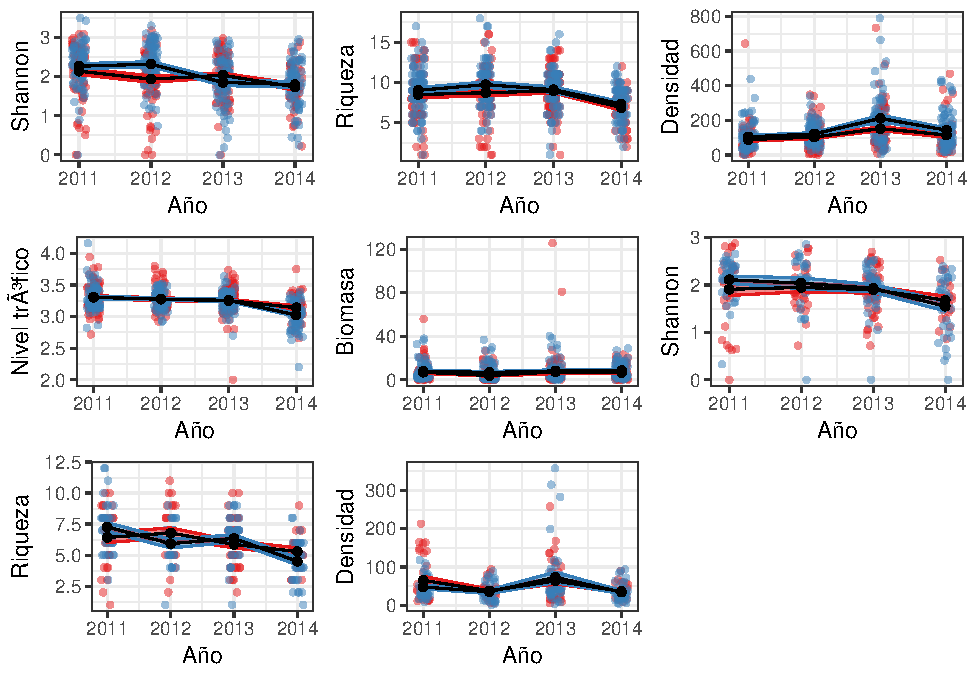
\includegraphics{Manuscript_files/figure-latex/unnamed-chunk-9-1.pdf}

\subsection{Maria Elena}\label{maria-elena}

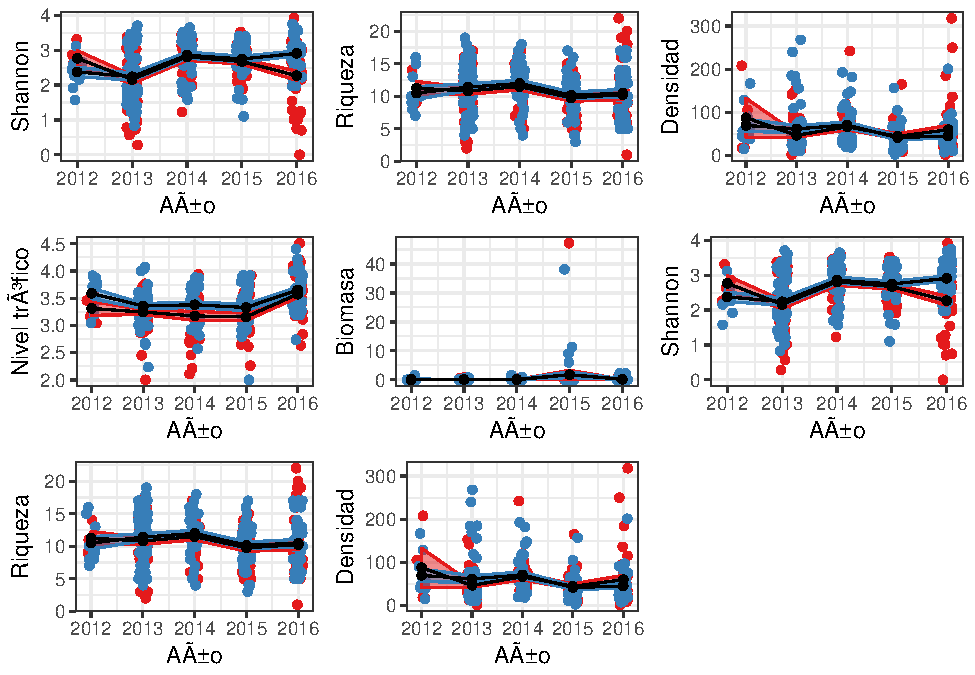
\includegraphics{Manuscript_files/figure-latex/unnamed-chunk-10-1.pdf}

\subsection{Punta Herrero}\label{punta-herrero}

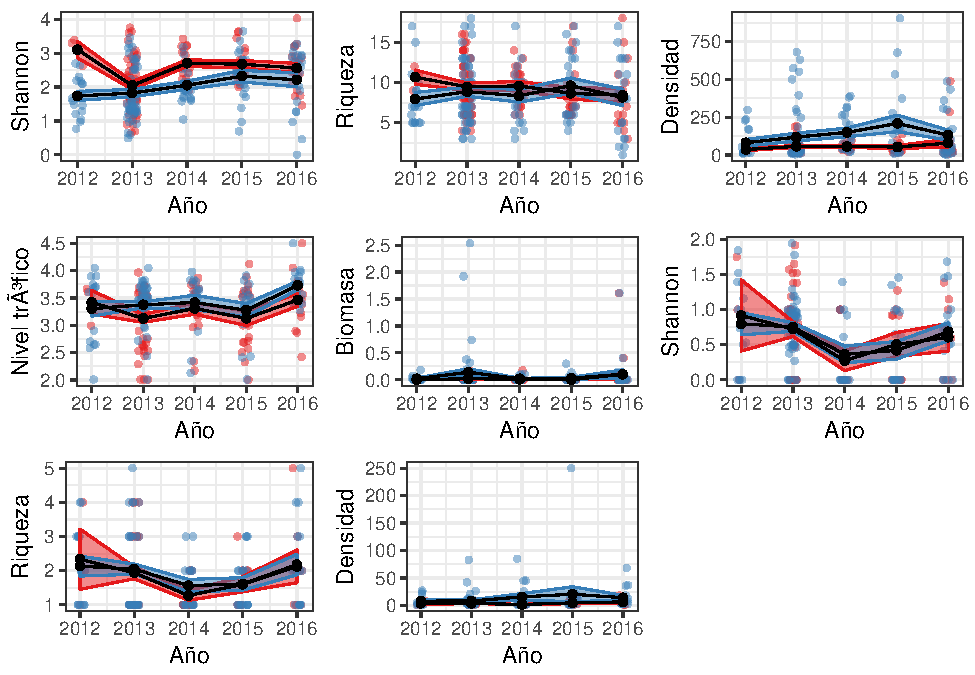
\includegraphics{Manuscript_files/figure-latex/unnamed-chunk-11-1.pdf}

\subsection{Efectos generales}\label{efectos-generales}

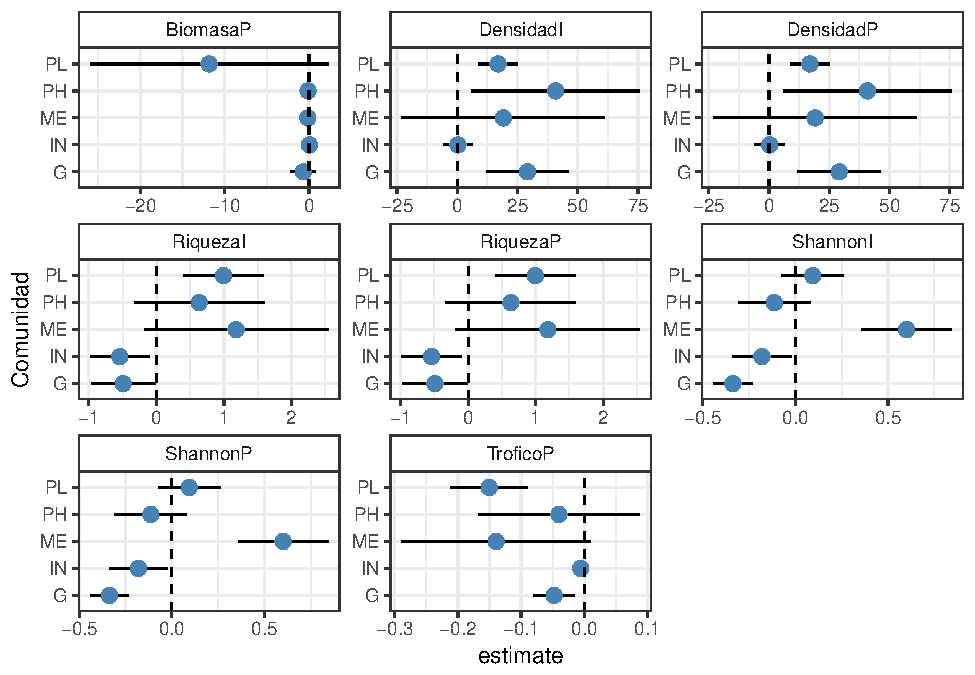
\includegraphics{Manuscript_files/figure-latex/unnamed-chunk-12-1.pdf}

\section{Conclusiones}\label{conclusiones}

\section*{Referencias}\label{referencias}
\addcontentsline{toc}{section}{Referencias}

\hypertarget{refs}{}
\hypertarget{ref-afflerbach_2014-HP}{}
Afflerbach, J.C., Lester, S.E., Dougherty, D.T. \& Poon, S.E. 2014. A
global survey of -reserves, territorial use rights for fisheries coupled
with marine reserves. \emph{Global Ecology and Conservation}. 2:97--106.
DOI:
\href{https://doi.org/10.1016/j.gecco.2014.08.001}{10.1016/j.gecco.2014.08.001}.

\hypertarget{ref-beger_2004-Y8}{}
Beger, M., Harborne, A.R., Dacles, T.P., Solandt, J.-L. \& Ledesma, G.L.
2004. A framework of lessons learned from community-based marine
reserves and its effectiveness in guiding a new coastal management
initiative in the philippines. \emph{Environ Manage}. 34(6):786--801.
DOI:
\href{https://doi.org/10.1007/s00267-004-0149-z}{10.1007/s00267-004-0149-z}.

\hypertarget{ref-difranco_2016-Xw}{}
Di Franco, A., Thiriet, P., Di Carlo, G., Dimitriadis, C., Francour, P.,
Gutiérrez, N.L., Jeudy de Grissac, A., Koutsoubas, D., et al. 2016. Five
key attributes can increase marine protected areas performance for
small-scale fisheries management. \emph{Sci Rep}. 6(1):38135. DOI:
\href{https://doi.org/10.1038/srep38135}{10.1038/srep38135}.

\hypertarget{ref-edgar_2014-UO}{}
Edgar, G.J., Stuart-Smith, R.D., Willis, T.J., Kininmonth, S., Baker,
S.C., Banks, S., Barrett, N.S., Becerro, M.A., et al. 2014. Global
conservation outcomes depend on marine protected areas with five key
features. \emph{Nature}. 506(7487):216--220. DOI:
\href{https://doi.org/10.1038/nature13022}{10.1038/nature13022}.

\hypertarget{ref-espinosaromero_2014-PY}{}
Espinosa-Romero, M.J., Rodriguez, L.F., Weaver, A.H., Villanueva-Aznar,
C. \& Torre, J. 2014. The changing role of ngos in mexican small-scale
fisheries: From environmental conservation to multi-scale governance.
\emph{Marine Policy}. 50:290--299. DOI:
\href{https://doi.org/10.1016/j.marpol.2014.07.005}{10.1016/j.marpol.2014.07.005}.

\hypertarget{ref-friedlander_2017-oI}{}
Friedlander, A.M., Golbuu, Y., Ballesteros, E., Caselle, J.E., Gouezo,
M., Olsudong, D. \& Sala, E. 2017. Size, age, and habitat determine
effectiveness of palau's marine protected areas. \emph{PLoS ONE}.
12(3):e0174787. DOI:
\href{https://doi.org/10.1371/journal.pone.0174787}{10.1371/journal.pone.0174787}.

\hypertarget{ref-gelcich_2015-Gw}{}
Gelcich, S. \& Donlan, C.J. 2015. Incentivizing biodiversity
conservation in artisanal fishing communities through territorial user
rights and business model innovation. \emph{Conserv Biol}.
29(4):1076--1085. DOI:
\href{https://doi.org/10.1111/cobi.12477}{10.1111/cobi.12477}.

\hypertarget{ref-giakoumi_2017-V2}{}
Giakoumi, S., Scianna, C., Plass-Johnson, J., Micheli, F.,
Grorud-Colvert, K., Thiriet, P., Claudet, J., Di Carlo, G., et al. 2017.
Ecological effects of full and partial protection in the crowded
mediterranean sea: A regional meta-analysis. \emph{Sci Rep}. 7(1):8940.
DOI:
\href{https://doi.org/10.1038/s41598-017-08850-w}{10.1038/s41598-017-08850-w}.

\hypertarget{ref-halpern_2017-Zi}{}
Halpern, B.S., Frazier, M., Afflerbach, J., O'Hara, C., Katona, S.,
Stewart Lowndes, J.S., Jiang, N., Pacheco, E., et al. 2017. Drivers and
implications of change in global ocean health over the past five years.
\emph{PLoS ONE}. 12(7):e0178267. DOI:
\href{https://doi.org/10.1371/journal.pone.0178267}{10.1371/journal.pone.0178267}.

\hypertarget{ref-halpern_2008-dK}{}
Halpern, B.S., Walbridge, S., Selkoe, K.A., Kappel, C.V., Micheli, F.,
D'Agrosa, C., Bruno, J.F., Casey, K.S., et al. 2008. A global map of
human impact on marine ecosystems. \emph{Science}. 319(5865):948--952.
DOI:
\href{https://doi.org/10.1126/science.1149345}{10.1126/science.1149345}.

\hypertarget{ref-hastings_2017-sm}{}
Hastings, A., Gaines, S.D. \& Costello, C. 2017. Marine reserves solve
an important bycatch problem in fisheries. \emph{Proc Natl Acad Sci U S
A}. (August, 9). DOI:
\href{https://doi.org/10.1073/pnas.1705169114}{10.1073/pnas.1705169114}.

\hypertarget{ref-krueck_2017-J1}{}
Krueck, N.C., Ahmadia, G.N., Possingham, H.P., Riginos, C., Treml, E.A.
\& Mumby, P.J. 2017. Marine reserve targets to sustain and rebuild
unregulated fisheries. \emph{PLoS Biol}. 15(1):e2000537. DOI:
\href{https://doi.org/10.1371/journal.pbio.2000537}{10.1371/journal.pbio.2000537}.

\hypertarget{ref-lester_2009-Ks}{}
Lester, S., Halpern, B., Grorud-Colvert, K., Lubchenco, J., Ruttenberg,
B., Gaines, S., Airamé, S. \& Warner, R. 2009. Biological effects within
no-take marine reserves: A global synthesis. \emph{Mar. Ecol. Prog.
Ser.} 384:33--46. DOI:
\href{https://doi.org/10.3354/meps08029}{10.3354/meps08029}.

\hypertarget{ref-micheli_2012-EU}{}
Micheli, F., Saenz-Arroyo, A., Greenley, A., Vazquez, L., Espinoza
Montes, J.A., Rossetto, M. \& De Leo, G.A. 2012. Evidence that marine
reserves enhance resilience to climatic impacts. \emph{PLoS ONE}.
7(7):e40832. DOI:
\href{https://doi.org/10.1371/journal.pone.0040832}{10.1371/journal.pone.0040832}.

\hypertarget{ref-nom049sagpesc_2014-V6}{}
NOM-049-SAG/PESC. 2014. NORMA oficial mexicana nom-049-sag/pesc-2014,
que determina el procedimiento para establecer zonas de refugio para los
recursos pesqueros en aguas de jurisdicción federal de los estados
unidos mexicanos. \emph{DOF}.

\hypertarget{ref-roberts_2017-J9}{}
Roberts, C.M., O'Leary, B.C., McCauley, D.J., Cury, P.M., Duarte, C.M.,
Lubchenco, J., Pauly, D., Sáenz-Arroyo, A., et al. 2017. Marine reserves
can mitigate and promote adaptation to climate change. \emph{Proc Natl
Acad Sci U S A}. 114(24):6167--6175. DOI:
\href{https://doi.org/10.1073/pnas.1701262114}{10.1073/pnas.1701262114}.

\hypertarget{ref-sala_2017-69}{}
Sala, E. \& Giakoumi, S. 2017. No-take marine reserves are the most
effective protected areas in the ocean. \emph{ICES Journal of Marine
Science}. DOI:
\href{https://doi.org/10.1093/icesjms/fsx059}{10.1093/icesjms/fsx059}.

\hypertarget{ref-uribe_2010-u2}{}
Uribe, P., Moguel, S., Torre, J., Bourillon, L. \& Saenz, A. 2010.
\emph{Implementación de reservas marinas en méxico}. 1st ed. (nos.).
Mexico.


\end{document}
